
%(BEGIN_QUESTION)
% Copyright 2012, Tony R. Kuphaldt, released under the Creative Commons Attribution License (v 1.0)
% This means you may do almost anything with this work of mine, so long as you give me proper credit

En instrumenttekniker prøver å kalibrere en reguleringsventil som del av et split-range-system, der ventilen skal være helt stengt ved 4 mA signal og helt åpen ved 9 mA signal:

$$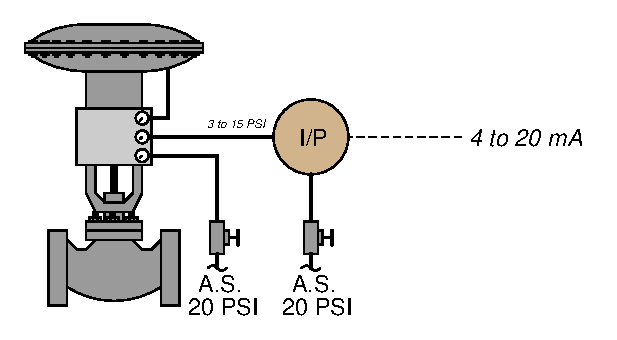
\includegraphics[width=15.5cm]{i01352x01.eps}$$

Dessverre klarer ikke posisjoneren på denne ventilen dette smale området: selv med ventilvandring-justeringen (span) justert helt til maksimum, krever ventilen 10.3 mA for å bli helt åpen, i stedet for ønsket 9 mA. Den klarer imidlertid å bli helt stengt ved 4 mA.

\vskip 10pt

Teknikeren ber kolleger om hjelp. Forslagene spenner fra å løsne fjærjusteringsmutteren på ventilaktuatorens stempelstang, til å øke luftforsyningstrykket til posisjoneren, til å justere posisjonerens ``zero''-skrue, til å installere en volume booster mellom posisjoneren og aktuatorens membran.

Utform din egen løsning på dette områdeproblemet for ventilen, og vær så konkret som mulig i svaret. Forklar også hvorfor ett av forslagene fra kollegene ikke vil løse problemet.

\underbar{file i01352}
%(END_QUESTION)





%(BEGIN_ANSWER)

Jeg anbefaler å gi 5 poeng for korrekt svar, og 5 poeng for korrekt avkrefting av ett av de foreslåtte tiltakene.

\vskip 10pt

Kanskje den enkleste løsningen her er å justere spennvidden (span) på I/P-en. Hvis ventilposisjoneren oppnår helt åpen ved 10.3 mA signal (7.725 PSI fra I/P-en), bør I/P-ens span justeres slik at den gir dette trykket ved 9 mA i stedet for 10.3 mA. Med andre ord bør I/P-kalibreringen være: {\bf 4 mA = 3 PSI} og {\bf 9 mA = 10.3 PSI}. Dette tilsvarer et I/P-utgangssignal på 26.36 PSI ved 20 mA.

\vskip 10pt

Å løsne fjærjusteringsmutteren vil ikke påvirke posisjonerens kalibrering, og enda verre: det vil redusere setelasten som er nødvendig for tett avstengning. Å øke posisjonerens luftforsyningstrykk kan hjelpe en posisjonerer med å oppnå helt åpen på en ventil med høyere øvre bench-set-verdi, men siden vi allerede klarer helt åpen, er ikke dette problemet her, og høyere forsyningstrykk er derfor ingen løsning. Justering av zero-skruen kan få ventilen til å bli helt åpen ved 9 mA, men da vil det kreves mindre enn 4 mA for å stenge (dvs. det løser ikke span-problemet). Til slutt vil en volume booster bare gjøre at ventilen posisjoneres raskere, men den påvirker ikke posisjonerens arbeidsområde.

%(END_ANSWER)





%(BEGIN_NOTES)

{\bf Dette spørsmålet er ment kun for eksamener, ikke for arbeidsark!}.

%(END_NOTES)

